\mysubsection{Choix des robots}
Il existe deux emplois différents à faire par des robots : la palettisation et le remplissage des caisses avec des bouteilles.\\
  
Dans les spécifications du projet, pour la palettisation est prévue que le préhenseur en charge aurait le poids de 25.8 kg et le robot choisi doit supporter cette charge. De plus, le bras du robot devra atteindre la zone des caisses et de palettes, ainsi il devra avoir un rayon d’action minimum égal le milieu du segment que relie les deux zones et aussi  le milieu du segment de la hauteur des caisses sur le convayeur et la zone des caisses , équivalent à 2075mm.La figure dessous représente ce calcul: \\

\begin{figure}[H]
	\begin{center}	
		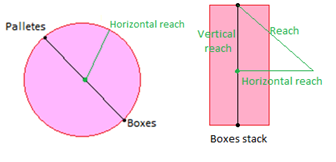
\includegraphics[width=8cm]{./Karol/Calculo.png}
		\caption{Répresentation du calcul de rayon d'action}
		\label{fig:representation}
	\end{center}
\end{figure}

Pour le remplissage des caisses avec des bouteilles est prévu que le préhenseur en charge aurait le poids de 5.47 kg et le bras du robot devra atteindre la zone des convoyeurs de bouteilles et des caisses, de la même façon que le robot antérieur, ce robot devra avoir un rayon d’action minimum égal le milieu du segment de relie les deux zones, équivalente a 414mm. 

\pagebreak
Alors, à partir de ces spécifications et considérant les meilleurs coûts-bénéfices en termes de production ont été choisis les robots suivants : \\




\underline{Robot de palettisation: robot controller 1}\\

\begin{figure}[H]
	\begin{center}	
		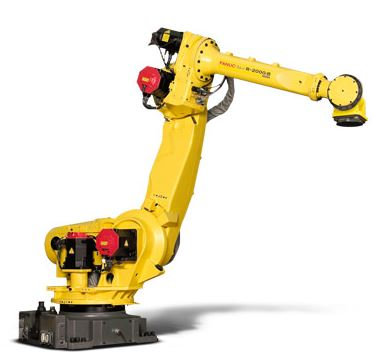
\includegraphics[width=8cm]{./Karol/figura1.JPG}
		\caption{Modèle: R-2000iB/100H-2}
		\label{fig:R-2000iB/100H-2}
	\end{center}
\end{figure}

\begin{itemize}
	\item Capacité de charge maxime admissible au poignet : 100 kg
	\item Rayon: 2655mm
	\item Axes: 5
\end{itemize}
\vspace{10pt}

Les autres robots de la série R-2000iB ont plus grande capacité de charge et rayon d’action, ainsi ils ont aussi plus grands coûts. Pourtant, parmi les robots de palettisation de cette série que répond aux spécifications du projet, c’est le robot avec le plus grand coût-bénéfice. \\

\underline{Robot de remplissage des caisses avec des bouteilles: robot controller 2 and 3 }\\


\begin{figure}[H]
	\begin{center}	
		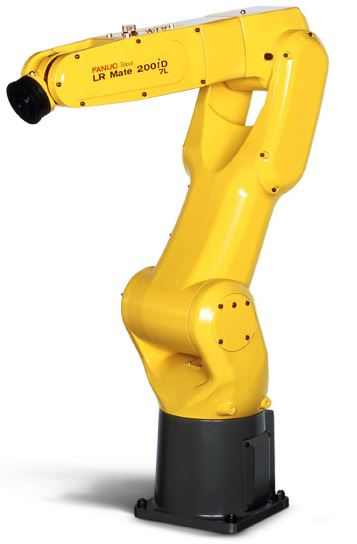
\includegraphics[width=4cm]{./Karol/figura2.JPG}
		\caption{Modèle: LR Mate 200iD/7L}
		\label{fig:LR_Mate_200iD/7L}
	\end{center}
\end{figure}
\newpage
\begin{itemize}
	\item Capacité de charge: 7 kg;
	\item Rayon: 911mm
	\item Axes: 6
	\item Bras long
\end{itemize}

\vspace{20pt}
Pour cette finalité, tout le robot poli articulé marche, mais la série LR Mate est spécifique pour robots plus petits et légers. Ainsi, c’est plus approprie pour les bouteilles. Un autre robot de cette série LR Mate 200iD/7LC a les mêmes spécifications techniques du robot choisi, mais il est de la line \textit{cleam room} robot, que il n’est pas nécessaire dans ce projet. Ainsi, pour répondre aux spécifications du projet le choix du robot LR Mate 2 – iD/7L est justifiée. \\
On a besoin de définir la quantité de robots. Pour remplissage des caisses avec des bouteilles, on a quatre bouteilles en 1.5s (sur chaque convoyeur). En considérant que le convoyeur doit être arrêté dans le moment que le robot prise les bouteilles, on doit ajouter le temps de prise. Ainsi, huit bouteilles prennent 1.75s. À partir de la simulation, en considérant la vitesse nominale, on trouve que le cycle complet du robot (20 bouteilles par caisse) prends 12.5s, c’est équivalent à 2.5s par quatre bouteilles. Avec ça, on peut conclure qu’on a besoin de deux robots pour le remplissage des caisses avec des bouteilles, parce qu’un unique robot ne serais pas suffisant pour répondre aux cadences des bouteilles et plus qu’un laissera le robot inoccupé pour une grande période. \\
On sait que deux caisses sont remplies avec des bouteilles en 12.5s. De plus, on peut ajouter 2s relatif au pas de deux caisses. Pourtant, le flux est des deux caisses en 14.5s, c’est équivalent à 7.25s pour chaque caisse. En considérant le temps technologique de prise et dépose, la palettisation prend le temps de 5.55s. C’est un temps possible pour le robot, ainsi on peut choisir seulement un robot de palettisation. 
 
